%=======================================================================
\section{Array Component} \label{s:component-array}
%=======================================================================

The \code{Array} classes encapsulate Fortran-style distributed or
vectorized arrays with convenient operations and optional special
features.

Optional features include storing as a blocked array to improve cache
use, array padding to avoid cache thrashing on large power-of-two
arrays with low-associativity caches.  Arrays also may be parallelized
according to \code{Parallel} objects such as
\code{Parallel::Mpi} for MPI-parallel distributed arrays, or
\code{Parallel::Omp} for OpenMP-parallel threaded arrays (or both).

The Array component is used to represent the concept of a
Fortran-style 3D array, but with data distributed or threaded in
various ways. Tentative functionality includes the following:

\begin{itemize}
\item Related groups of 1-, 2-, 3-D style Fortran arrays
\item MPI-distributed arrays
\item OMP-threaded array
\item UPC-distributed arrays
\item Hybrid distributed/threaded arrays
\item Efficient iterators over array blocks for computations
\item Parallelization and data distribution are hidden in block
  iterators
\item Support for both permanent and allocate-when-needed ghost zones
\item Efficient resizing / combining / merging functions for
  integration with Mesh
\item Efficient transposing / permuting of axes, e.g. for PPM to
  compute with stride-1 along all axes
\item Efficient ghost-zone refresh
\item Group operations for controlling relative data layout of
  multiple arrays
\item Support for cell-centered, face-centered, edge-centered, or
  corner storage
\item Optional blocked storage for improved cache use or vector
  behavior
\item Optional padding for low-associativity caches
\end{itemize}

To implement Array's, other related classes are used to share implementation responsibilities. These classes are described in separate pages.

\begin{description}
\item [Layout] The Layout class is used to define an Array's
  configuration, but does not allocate any data. Array's that share
  the same Layout object are said to be conforming. An Array's Layout
  describes how to distribute an Array's data over MPI processes,
  between OpenMP threads, etc. For unigrid problems, only one Layout
  is used. For AMR problems, typically several Layouts are used.

\item [Block] The Block class is a lightweight wrapper for portions of
  an Array to be actively computed by a single thread. It represents a
  Fortran-style array, together with offset, stride, dimension, and
  size.

\item [ItBlock] The ItBlock class is used to iterate over Block's of
  Array's that share conforming Layout's.
\end{description}

\subsubsection{Issues}

Issues with Arrays and supporting classes include the following:

\begin{itemize}
\item How to handle iterators in a way that the calling code doesn't
  know what Layout varieties are used
\item How to handle nested iterators in calling code for hybrid
  parallelization Layouts
\item How to handle load balancing
\item How to communicate between array blocks to refresh ghost zones
\item How to communicate between arrary blocks for interpolation
\item How to handle permanent versus temporary ghost zones
\item How to support cell-, face-, edge-centered variables in same
  layout
\item How to control layout within a Layout, e.g. interleave range of
  arrays but not others.
\end{itemize}

\subsubsection{Operations}

\begin{itemize}
\item Allocation and deallocation functions (Memory)
\item Copy functions
\item Merge / split functions (for AMR)
\item Universal properties functions for obtaining information about
  the array (dimensions, etc.)
\item Layout-dependent properties (MPI task distribution, cache block
  sizes, etc.)
\item Iterators for looping over array blocks
\item Reshape / resize functions for converting between different
  array configurations (blocked to unblocked, with ghosts to without
  ghosts, etc.)
\item Accessor functions for neighboring values
\item Refresh functions for obtaining updated ghost zone values
  (accesses Parallel)
\item I/O functions (Disk)
\end{itemize}

\subsection{\code{Array}}

\centerline{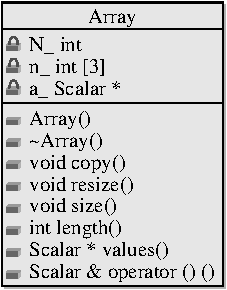
\includegraphics{uml/array.pdf}}

\subsubsection{Array shape}

\subsubsection{Array blocking}

\subsubsection{Array padding}

\subsubsection{Array interleaving}


\subsection{Attributes}

\begin{tabbing}
xx\=xx\=xxxxxxxxxxxxxxxxxxxxxxxxxxxxxxxxxxx\= \kill
\> \todo \>  \textit{Length of array} \\
\>       \> \code{N\_: int }      \\ \\
\> \todo \>  \textit {Shape of array, right-padded with 1's} \\
\>       \> \code{n\_: int [3] }  \\ \\
\> \todo \>  \textit {Array values stored in column-major ordering}\\
\>       \> \code{a\_: Scalar * }
\end{tabbing}

\subsection{Operations}

\begin{tabbing}
xx\=xx\=xxxxxxxxxxxxxxxxxxxxxxxxxxxxxxxxxxx\= \kill
\> \todo \> \textit{Create a new uninitialized Array object} \\
\>       \> \code{Array()} \\ \\
\> \todo \> \textit{Create a new initialized Array object} \\
\>       \> \code{Array(int n0, int n1=1, int n2=1, int n3=1)} \\ \\
\> \todo \> \textit{Deallocate the array} \\
\>       \> \code{\~{\ }Array()}  \\ \\
\> \todo \> \textit{Copy an array into this one, deallocating any existing data} \\
\>       \> \code{void copy (const Array \&)}  \\ \\
\> \todo \> \textit{Resize the array, deallocating any existing data} \\
\>       \> \code{void resize (int n0, int n1=1, int n2=1, int n3=1)}   \\ \\
\> \todo \> \textit{Return the size of the array} \\
\>       \> \code{void size (int *n0, int *n1=0, int *n2=0, int *n3=0) const}  \\ \\
\> \todo \> \textit{Return the total length of the array} \\
\>       \> \code{int length () const}  \\ \\
\> \todo \> \textit{Return a pointer to the array values} \\
\>       \> \code{Scalar * values () const}  \\ \\
\> \todo \> \textit{Return the given array element} \\
\>       \> \code{Scalar \& operator () (int i0, int i1=0, int i2=0, int i3=0)}
\end{tabbing}


